\section{Methodology}
\label{sec:methodology}

In this section, we introduce key steps of our works. We first detail how the architecture of SketchPointNet is designed. Next, we will show how to resample each sketch into a fixed number of points. At last, we explain that our group scheme guarantees the integrity of each group patterns.

\subsection{SketchPointNet}
\label{ssec:sketch_point_net}

SketchPointNet architecture(see Fig.~\ref{fig:sketchpointnet}) are borrowed from PointNet++ architecture. The differences between SketchPointNet and PointNet++ are how we select group centers and group the points. For PointNet++, they use iterative farthest point sampling to choose group centers to ensure that group centers are evenly distributed. Sketch points are sparsely distributed on the strokes. We choose group centers every $t$ points along the time series(each sketch represented as a time series). The way we choose group centers is faster the way in PointNet++. In a meanwhile,
our group centers are nearly evenly distributed in 2d space. When group the point around group centers, we have to set a proper group numbers. In PointNet++, if the group numbers is greater than setting group number, they directly delete last extra points. But we delete points every other points till the group number equals to setting group number. This can ensure the integrity of the pattern(see Fig. ~\ref{fig:group}).

In order to get local pattern information of each sketch, we group sketches for two times. Micro PointNet P1 summarize patterns with group radius $r_1$ equals to 0.1. Micro PointNet P2 summarize patterns in a large receptive field with $r_2 = 0.3$. PointNet P3 summarize pattern features generated from m2 for classification of 250 categories.

In detail, each sketch is represented as 1024 points. Each point has 3 dimension. The first two dimension denote the location of the point. The last dimension is the stroke order information(each point belong to a stroke). In order to extract features of local patterns, we resample 512 points as group center every other points and group the points around the group center with $r_1 = 0.1$. After the first time of grouping, we get 512 groups $\left\{ g_{1_i}| i = 1, ..., 512 \right\}$. Each group contains 20 points. We get a 5d pattern feature after each of 512 groups passing through the micro PointNet P1. The feature of each group is a 8d vector which contains two parts. The first 5 dimension indicate the pattern feature of the group. The last 3 dimension indicate the center location of the group.

In a similar way, we resample points every 4 points from the last group centers. Then we get 128 larger groups $\left\{ g_{2_i}| i = 1, ..., 128 \right\}$ after grouping $g_1$ with $r_2 = 0.3$. Each larger group contains 128 smaller groups from $g_1$. We get 29d vector as $g_2$ pattern features after feeding 128 smaller groups $g_1$ into micro PointNet P2. Pattern features concated with its center location are group features for each of $g_2$. At last, we feed PointNet P3 with $g_2$ group features. SketchPointNet output 250 scores corresponding to 250 categories.

\begin{figure}
    \center
    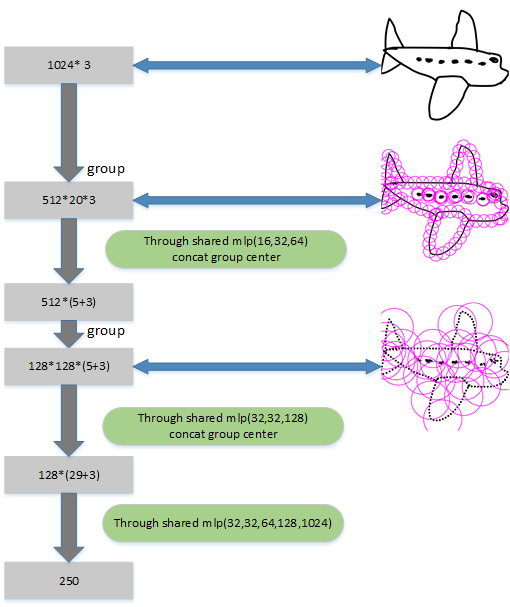
\includegraphics[width=3in]{images/sketchpointnet.png}
    \fcaption{SketchPointNet architecture.}
    \label{fig:sketchpointnet}
\end{figure}


\subsection{Resample scenario}
\label{ssec:resample_scenario}

For each sketch, we sample it into a fixed number of points. Or we can sample each points in sketches with a given interval. In second case, the point number $\left\{ N_{P_i}| i = 1, ..., 20000 \right\}$ of sketches are different due to various total stroke length of each sketch. The input to the network must have a fixed size. Because tensorflow 1.2 only support static graph. If we set input size as $\max \limits_{1 \le i \le 20000} N_{P_i}$, there are great waste for computing resources. Because only few sketches need large input size.

\begin{figure}
    \center
    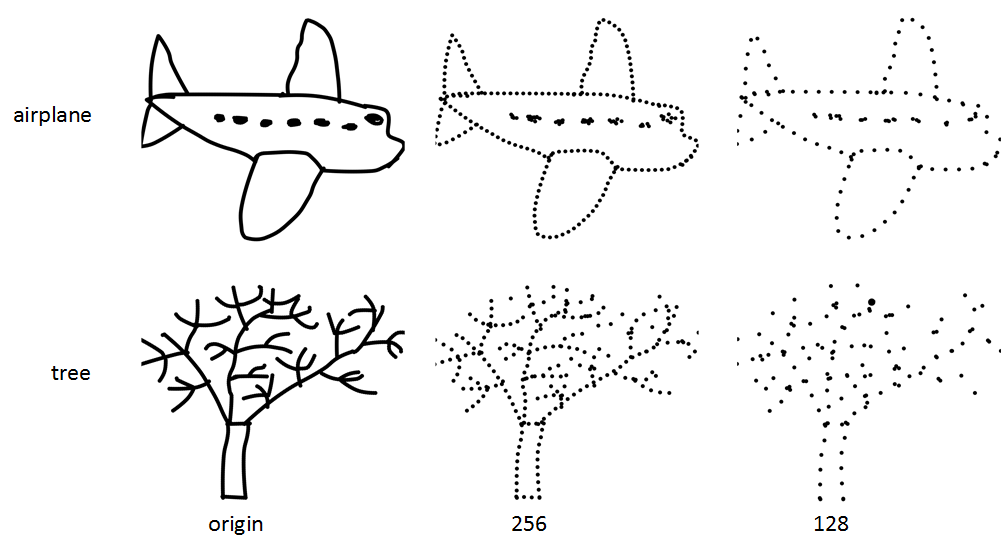
\includegraphics[width=3in]{images/resample2.png}
    \fcaption{Resample the airplane and the tree into $N$(256 and 128) points.}
    \label{fig:resample}
\end{figure}

 We calculate each stroke length $\left\{ L_i| i = 1, ..., m \right\}$ from strokes $\left\{ T_i^{init}| i = 1, ..., m \right\}$. $m$ stands for stroke numbers. The total stroke length is $C$. Given the number of points $N$, we assign each stroke $B_i$ points $\left\{ B_i| i = 1, ..., m \right\}$ according to its corresponding stroke length $T_i$. Then we reample each stroke in $B_i$ points by using \$1 \cite{Wobbrock2007GesturesWL} resample scheme. The strokes after resampled are represented as $\left\{ T_i^{rsp}| i = 1, ..., m \right\}$. In Fig.~\ref{fig:resample}, the airplane and the tree are resample into different number of points.
 
\begin{algorithm}
\label{alg:resample}
    \caption{Resample each sketch into N points}
    \KwIn{$\left\{ T_i^{init}| i = 1, ..., m \right\}$, resample number $N$}
    \KwOut{$\left\{ T_i^{rsp}| i = 1, ..., m \right\}$}
    $C = 0$\;
    \For{$ i = 1; i \le m $}
    {
        $L_i = |T_i^{init}|$\;
        $C = C + L_i$\;
    }

    \For{$ i = 1; i \le m $}
    {
        $B_i = \frac{L_i \times N}{C}$\;
        $T_i^{rsp} = single\_stroke\_resample(T_i^{init}, B_i)$\;
    }
    return $\left\{ T_i^{rsp}| i = 1, ..., m \right\}$\;
\end{algorithm}



\subsection{Group scheme}
\label{ssec:group_scheme}

After resampling sketches, we get each of them represented as N points $\left\{P_i| i = 1,..., N\right\}$. For a sketch, We resample a series of points $\left\{P_{1}, P_{1+t}, P_{1+2*t}, ..., P_{1+(N_g-1)*t}\right\}$ every $t$ points as group center from the N Points. Then we group points according to group center with radius $r$. After grouping the sketch, we get $N_{g} \times S_{g}^{init}$. $N_{g}$ is the number of the groups. $S_{g}^{init}$ is the points number of each group. In a similar way, we group the sketch for more times according to last grouping center.

The input group must have a fixed point number $S_g$. But with a fixed group radius $r$, group point numbers are very different from each other. After grouping the points, We get a series of groups. One of the groups contains $S_g^{init}$ group points $\left\{ Z_i| i = 1, ..., S_g^{init} \right\}$. If the point number $S_g^{init}$ is less than $S_{g}$, we pad the group center into the group till the group size is $S_{g}$. If the point number $S_g^{init}$ is greater than $S_{g}$, we delete group points every other points in the group till the point numbers is $S_{g}$. We develop an algorithm to guarantee the integrity of group patterns when deleting extra points.

\begin{algorithm}
\label{alg:group}
    \caption{Delete extra points until group size is $S_g$}
    \KwIn{$\left\{ Z_i^{init}| i = 1, ..., m \right\}$, group size threshold $S_g$}
    \KwOut{$\left\{ Z_i| i = 1, ..., S_g \right\}$}
    $i = 2$\;
    $Z = Z^{init}$\;
    \While{$|Z| < S_g$}
    {
        \If{$i = |Z|+1$ or $i = |Z|+2$}
        {
            $i = 2$\;
        }
        del $Z_i$\;
        $i = i+1$\;
    }
    return $\left\{ Z_i| i = 1, ..., S_g \right\}$\;
\end{algorithm}

\begin{figure}
    \center
    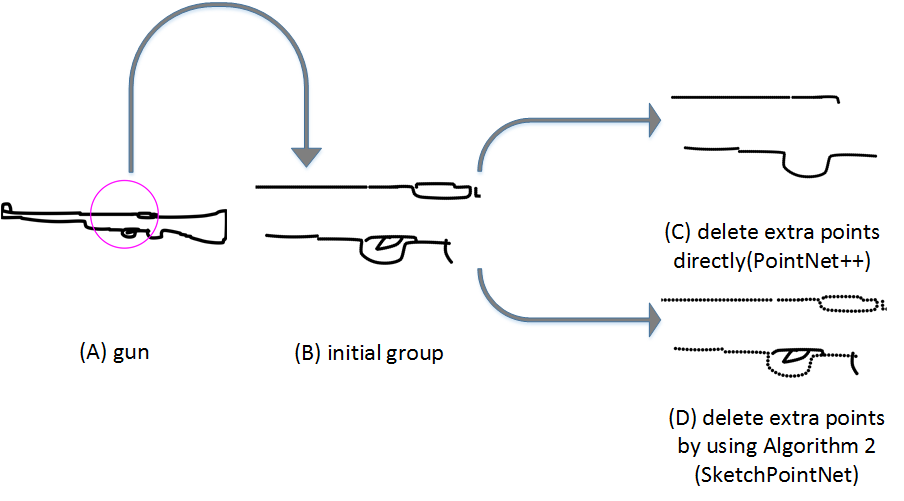
\includegraphics[width=3in]{images/group.png}
    \fcaption{Comparison of dealing with extra points.}
    \label{fig:group}
\end{figure}

All N points in a sketch are chronological. Grouping do not undermine the order of time series. The points in a group are still arranged in chronological order. In Fig.~\ref{fig:group} (B), The initial group contains $S_g^{init}$ points which is greater than $S_g$ points. If we directly delete the last $|S_g^{init}-S_g|$ points. From Fig.~\ref{fig:group} (C), we can see that there are great loss of the pattern.  Algorithm ~\ref{alg:group} makes sure of the existence of the whole pattern(see Fig.~\ref{fig:group} (D)).


